%\chapter{det-overview}

%%%%%%%%%%%%%%%%%%%%%%%%%%%%%%%%%%%%%%%%%%%%%%
\section{Detector Requirements}

insert detector overview here

%%%%%%%%%%%%%%%%%%%%%%%%%%%%%%%%%%%%%%%%%%%%%%
\section{Liquid argon detector properties}
- Electron drift + LAr purity etc.
- LAr scintillation light 

%%%%%%%%%%%%%%%%%%%%%%%%%%%%%%%%%%%%%%%%%%%%%%
\section{TPC Signal Formation (Xin)}\label{sec:tpc_signal_formation}

The principle of the large single-phase LArTPC with wire readouts is shown in 
Fig.~\ref{fig:signal}. When charged particles traverse through the LAr medium,
ionization electrons are generated. They would travel at a constant speed 
($\sim$1.6 km/s at 500 V/cm electric field) along the external electric field 
toward the multiple anode wire planes. The first wire planes encountered collect 
an induction signals as the drifting charge passes through.  The charge is collected 
on the wires in the final plane. This transparency of the induction planes is assured by 
applying an appropriate bias voltage to these wire planes.
During this process, current will be produced on the wire planes. 
Since the locations of wires are accurately known, the position of the
ionization charge in the direction transverse to the drift can be determined in 
three independent views. The time of the initial interaction can be determined by collecting 
scintillation light 
in a fast optical detector system.
Measuring the time from this prompt activity to signals on the wires it is 
possible to determine the longitudinal position along the drift direction.
Therefore, one can achieve a 3D imaging of the trajectories of the charged particles in the LAr. 
The amount of ionization electrons depends on the energy and type of
the initial particles, and can be used to deduce their properties.

\begin{figure}[htb]
\centering
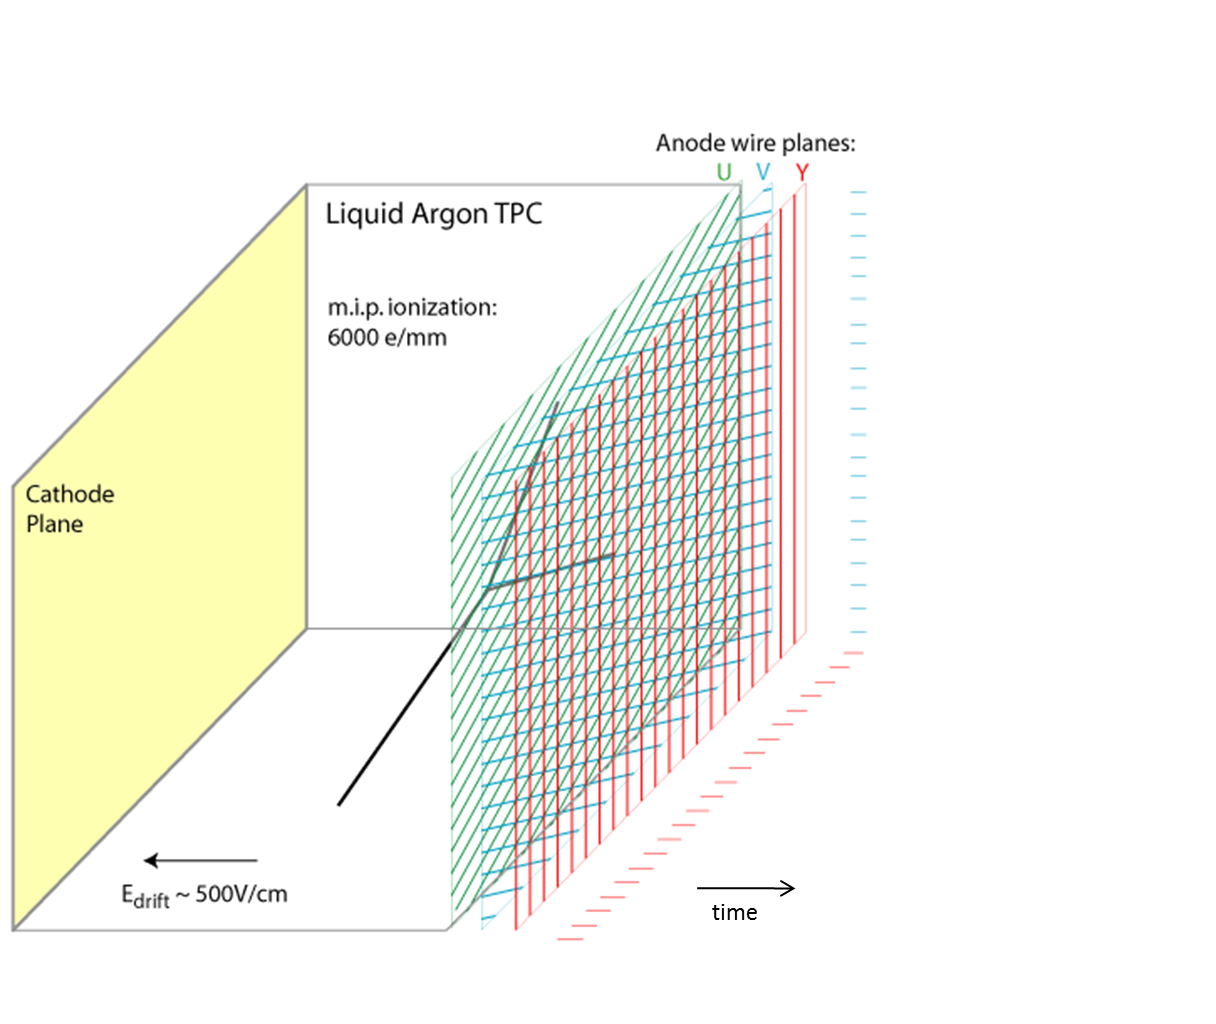
\includegraphics[width=0.48\textwidth]{figures/TPC_1.png}
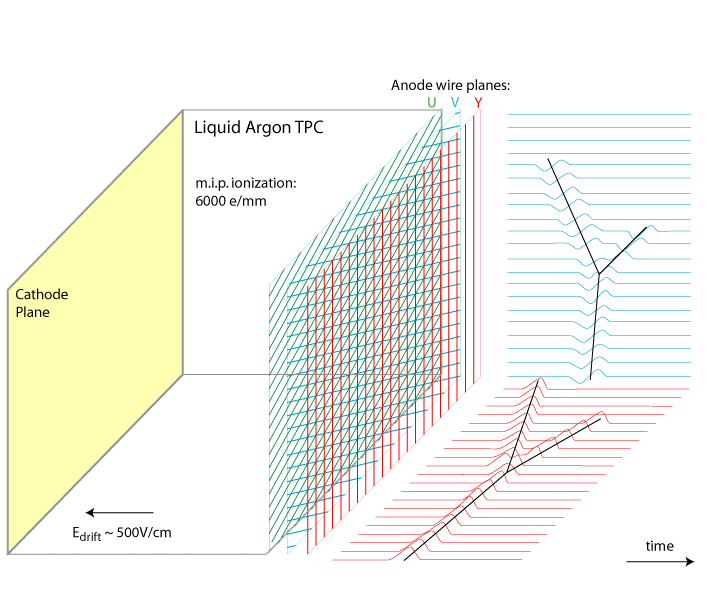
\includegraphics[width=0.48\textwidth]{figures/TPC_2.png}
\caption{The principles of LArTPC are shown. (left) When energetic, charged particles 
traverse the LAr medium, ionization electrons are produced and move
along the external electric field towards the anode planes. (right) The ionization
electrons pass through the induction wire planes and are  collected by the 
final collection wire plane. 
During this process, signals are measured on the wires
in each plane which provides information about the 3D positions and
energies of initial particles.}
\label{fig:signal}
\end{figure}

Figure~\ref{fig:signal_formation} illustrates the major elements of the  
processes involved in forming the TPC signals. 
When the ionization electrons drift through the wire planes, current is 
induced on the nearby wires. This process is described by the field response
functions. The physics of the current induction is described by the Shockley-Ramo 
theorem~\cite{Shockley,Ramo}.  For an element of ionization charge, 
the instantaneous, induced current $i$ is proportional to the amount of that
charge $q$ and its drifting velocity $v_q$:
\begin{equation}
i = q \cdot E_{weight} \cdot v_q.
\end{equation}
The proportionality factor is the weighting field $E_{weight}$ at the 
location of the charge. The weighting field $E_{weight}$ 
depends on the geometry of the electrodes. Figure~\ref{fig:signal_formation} shows a 
calculated weighting potential for one induction plane wire using a 2D simulation based 
on Garfield~\cite{garfield}. 
In this setup, the wire pitch is assumed to be 3 mm. There are three wire planes 
with the first two being induction and last one being collection plane. 

The induced current on the wire is received, amplified, and shaped by
a pre-amplifier. This part is described by the electronics response
function (see Fig.~\ref{fig:ele_res}).  
The resulting signal waveform is then digitally sampled at
regular intervals.  This data is referred to as the raw digits.  The
goal of the signal calibration process is to recover the number of
ionization electrons that must have arrived at each anode plane at a
given sample time in order to produce the measured raw digits.  The
information regarding the number, location (in the directions transverse
to and in the plane of the wires) and sample time of ionization
electrons are then used as input to the event reconstruction chain.

\begin{figure}[htb]
\centering
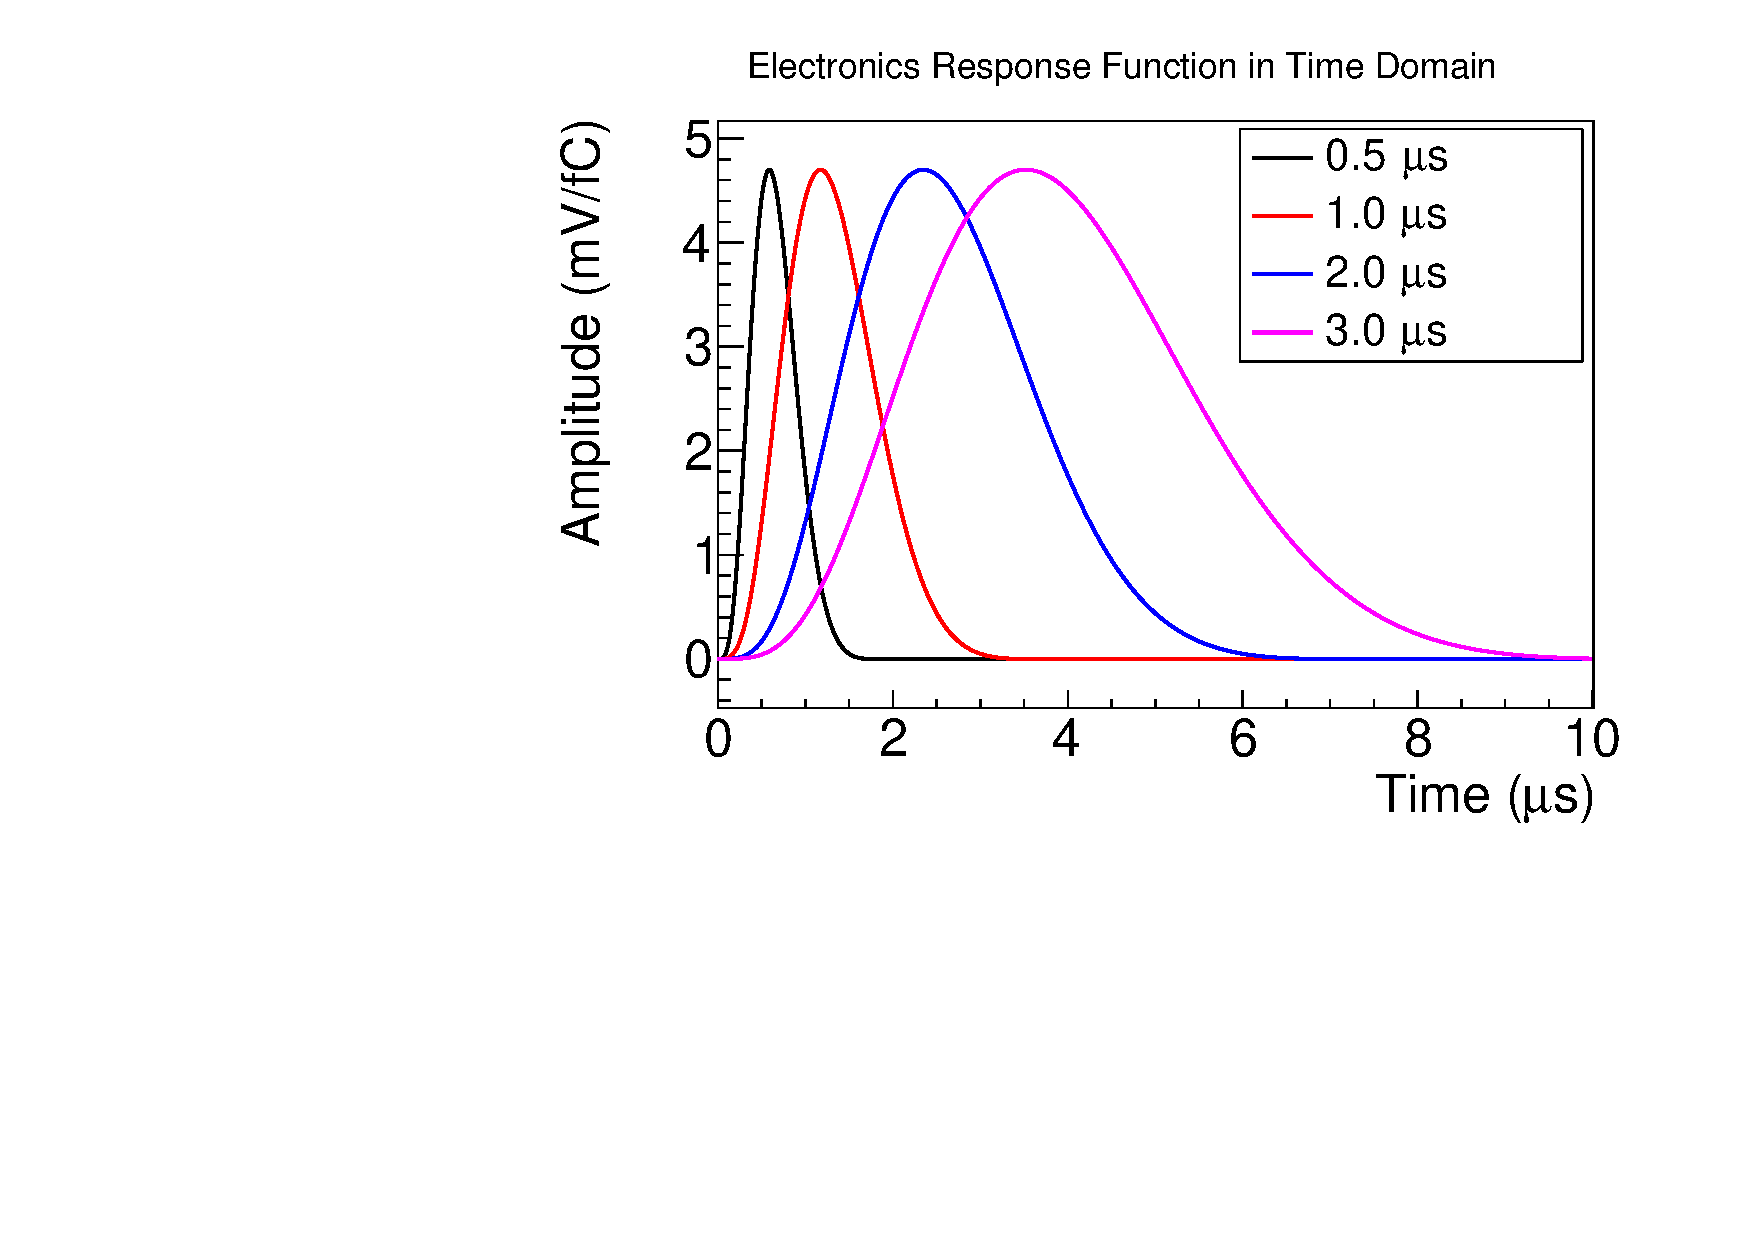
\includegraphics[width=0.8\textwidth]{figures/electronics_res.pdf}
\caption{The simulated electronics response function in the time domain at 4.7 mV/fC gain. 
The front-end cold electronics are designed to be programmable with 4 different 
gain settings (4.7, 7.8, 14, and 25 mV/fC) and 4 shaping time settings 
(0.5, 1, 2, and 3 us). The shaping time is defined as the time 
between peak and 5\% of the peak. For a fixed gain setting, the peak 
is always at the same height independent of the shaping time. }
\label{fig:ele_res}
\end{figure}



\begin{figure}[htb]
\centering
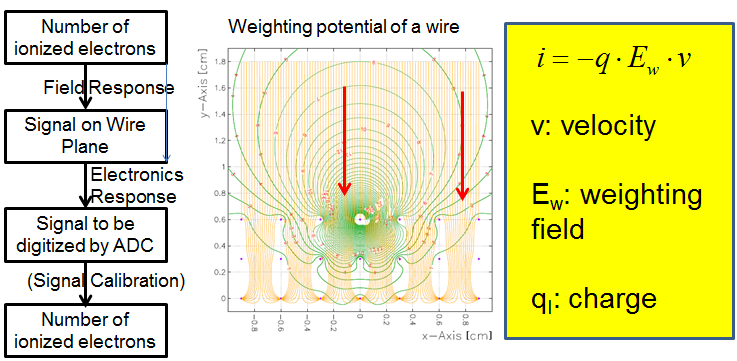
\includegraphics[width=0.8\textwidth]{figures/Signal_formation.png}
\caption{The process of TPC signal formation. See text for more explanations.
\textcolor{red}{This plot will be replaced with DUNE Garfield simulation ...}}
\label{fig:signal_formation}
\end{figure}

While the principle is straight forward, calculating the measured
current itself can be very complicated. As shown in
Fig.~\ref{fig:signal_formation}, the weighting field becomes smaller
at locations further away from the wire of interest.  
The weighting field also extends beyond the ``boundary'' of the wire.
Wire boundaries are defined by imaginary planes parallel to a wire,
perpendicular to the wire's plane and half way between two neighboring
wires.  That is, in an ideal case, all charge produced in a boundary
will drift nearest to its associated wire.
Due to the extent of the weighting field, electrons drifting inside
one wire's boundary can induce current in other wires.  This fact
makes the induced current strongly depend on the local ionization
charge distribution near the wire of interest, which in turn depends
on the event topology of the initial energetic, charged particles.


To illustrate the complication of the induction plane signal, we show an ideal track with a uniform charge 
distribution along the track as an example in Figure~\ref{fig:ideal_track_1}.
On the left panel, the two black lines represent the boundary of one wire region. In this case, 
if one just counts the ionization charge distribution within the wire region, the expected 
distribution is shown in the panel a) on the right.  However, the induced current on the wire of 
interest depends on the weighting field, which is smaller when the ionization electron is 
further away from the wire itself. Therefore, the effective charge distribution seen by 
the wire would be similar to the panel b) on the right side of 
Fig.~\ref{fig:ideal_track_1}. However, this is not the end of story. For ionization electrons 
drifting by in the near-by wires boundaries, the wire of interest will also experience a 
further induced current. In this case, since the ionization electrons are further away 
from the target wire, the weighting field is even smaller and thus their induction is 
also smaller. The realistic effective charge distribution will be similar to the panel c) on 
the right side of Fig.~\ref{fig:ideal_track_2}. 

We can then see what happens to the raw digits when we take into account the bipolar induction 
field response function. In the left panel of Fig.~\ref{fig:ideal_track_2}, the top half shows 
the real charge distribution going through the targeted wire region. The convolution of this 
distribution with a bipolar response function will lead to results shown at the bottom. In this 
case, we can see the signal height is still large at least for the start and the end of the 
signal. In the right panel of Fig.~\ref{fig:ideal_track_2}, the top half shows the more 
realistic effective charge distribution seen by the targeted wire. The convolution of this 
distribution with a bipolar response function will lead to results shown at the bottom. In 
this case, we can see that the signal height is much smaller though the length of signal is 
long. This effect leads to complications in designing the zero-suppression algorithm.


\begin{figure}[!h!tbp]
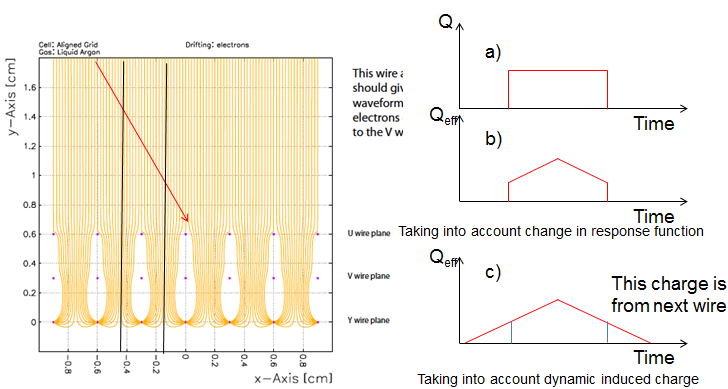
\includegraphics[width=0.95\textwidth]{figures/ideal_track.png}
\caption{Illustration of the induction plane field response for an ideal track. See text for more 
discussions. }
\label{fig:ideal_track_1}
\end{figure}

\begin{figure}[!h!tbp]
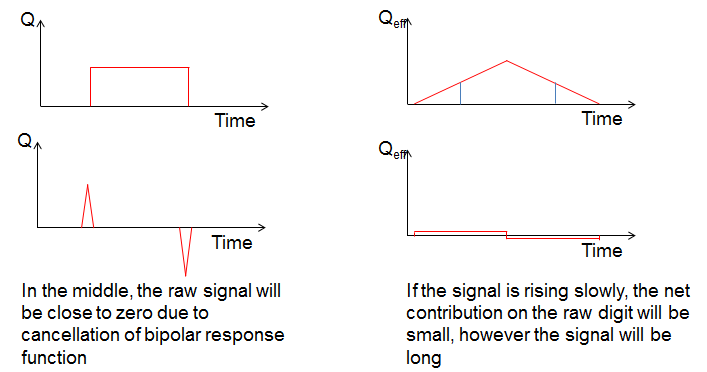
\includegraphics[width=0.95\textwidth]{figures/ideal_track_2.png}
\caption{Illustration of the induction plane field response for an ideal track. See text for more 
discussions.}
\label{fig:ideal_track_2}
\end{figure}



%%%%%%%%%%%%%%%%%%%%%%%%%%%%%%%%%%%%%%%%%%%%%%
\section{Space charge effects}

%%%%%%%%%%%%%%%%%%%%%%%%%%%%%%%%%%%%%%%%%%%%%%
\section{...}
